\section{Conditional Controls}
\begin{frame}<beamer>
    \frametitle{Outline}
    \tableofcontents[currentsection]
\end{frame}

\subsection{if-else clause}
\begin{frame}<beamer>
    \frametitle{Outline}
    \tableofcontents[currentsection, currentsubsection]
\end{frame}

\begin{frame}[fragile]{Start with a simple example}
\begin{itemize}
	\item {Guess what the following code for}
\end{itemize}
		\begin{lstlisting}
#include <stdio.h>
int main()
{
    int x = 5;
    if(x%2 == 0)
    {
       printf("x is an even number.");
    }
    return 0;
}
		\end{lstlisting}
\vspace{-0.15in}
\begin{itemize}
	\item {\textcolor{blue}{if} statement makes a judgement}
	\item {If the \textcolor{red}{logic/conditional} expression is \textcolor{red}{true}}
	\item {The statment(s) inside \{...\} will be executed}
	\item {Otherwise, statment(s) will be \textcolor{red}{ignored}}
\end{itemize}
\end{frame}

\begin{frame}[fragile]{Logic/conditional expression (1)}
\begin{itemize}
	\item {Let's now focus on the conditional expression}
\end{itemize}
		\begin{lstlisting}
#include <stdio.h>
int main()
{
    int x = 5;
    if(conditional_expression)
    {
       printf("x is an even number.");
    }
    return 0;
}
		\end{lstlisting}
\vspace{-0.15in}
\begin{itemize}
	\item {It is a expression that returns \textcolor{blue}{true} or \textcolor{blue}{false}}
	\item {For example, statement ``you are undergraduate student''}
	\item {We can judge whether it is true or false}
	\item {\textcolor{red}{Paradox}, story shared}
\end{itemize}
\end{frame}

\begin{frame}[fragile]{Logic/conditional expression (2)}
	\begin{itemize}
		\item {In C, expression with \textbf{relational operators} is used as conditional expressions}
		\item {They are}
		\begin{enumerate}
			\item {$<$, $>$, $<$=, $>$=}
			\item {== for ``equal to''}
			\item {!= for ``not equal to''}
		\end{enumerate}
		\item {It returns 1 (true) or 0 (false)}
	\end{itemize}
\begin{lstlisting}
int main()
{
    int a = 0, b = 0, c = 0;
    a = (3 > 5);
    b = (2*2 > 4);
    c = (3 == 3);
    return 0;
}
\end{lstlisting} 
\end{frame}

\begin{frame}[fragile]{Comments}
\vspace{-0.3in}
\begin{eqnarray}
p=\frac{-b}{2a}, & q=\frac{\sqrt{b^2-4ac}}{2a} \nonumber \\
x_1=p+q, & x_2=p-q \nonumber
\end{eqnarray}
\begin{itemize}
	\item {For the case ${b^2-4ac} < 0$}
	\item {We should output ``no real solution''}
	\item {For the case, ${b^2-4ac} \geq 0$}
	\item {We should output \textit{x1} and \textit{x2}}
\end{itemize}

\end{frame}

\begin{frame}[fragile]{Solve Quadratic Equation}
\vspace{-0.1in}
	\begin{columns}
		\begin{column}{0.1\linewidth}
		\end{column}
		\begin{column}{0.9\linewidth}
	\begin{lstlisting}[]
#include <stdio.h>
#include <math.h>
int main()
{
    float a = 0, b = 0, c = 0, delta = 0;
    float x1 = 0, x2 = 0, p = 0, q = 0;
    printf("Input a, b and c:\n");
    scanf("%f%f%f", &a, &b, &c);
    delta = b*b - 4*a*c;
    if(delta >= 0){
       p = -b/(2*a);
       q = sqrt(delta)/(2*a);
       x1 = p + q; x2 = p - q;
       printf("x1=%f, x2=%f\n", x1, x2);
    }else{
       printf("No real solution!\n");
    }
    return 0;
}
\end{lstlisting}
\end{column}
\end{columns}
\end{frame}

\begin{frame}[fragile]{Exercise}
\vspace{-0.3in}
	\begin{columns}
		\begin{column}{0.1\linewidth}
		\end{column}
		\begin{column}{0.9\linewidth}
	\begin{lstlisting}[linewidth=0.9\textwidth]
#include <stdio.h>
int main()
{
    int a = -1;
    unsigned int b = 600;
    if(a > b)
    {
        printf("%d is greater than %d\n", a, b);
    }else{
        printf("%d is smaller than %d\n", a, b);
    }
    return 0;
}
	\end{lstlisting}
	\end{column}
\end{columns}
\begin{itemize}
	\item {\textcolor{red}{What is the answer??}}
\end{itemize}
\end{frame}

\subsection{Logical operators}
\begin{frame}<beamer>
    \frametitle{Outline}
    \tableofcontents[currentsection, currentsubsection]
\end{frame}

\begin{frame}[fragile]{Logical Operators (1)}
\begin{itemize}
	\item {In some cases, single conditional statement is not enough}
	\item {For example, we want to express following condition}
	\item {If a $>$ b AND b $>$ c, then ...}
	\item {We need a way to connect several statements}
	\item {Usually, we use AND, OR and NOT}
	\item {In C, they are \&\&, $||$ and !}
\end{itemize}

\begin{itemize}
	\item {AND (c1 \&\& c2): means only when c1 and c2 both are true,  it is true}
	\item {OR (c1 $||$ c2): means when either c1 or c2 is true,  it is true}
	\item {NOT (!c1): means reverse it, c1 is true, !c1 is false; c1 is false, !c1 is true}
\end{itemize}

\end{frame}

\begin{frame}[fragile]{Logical Operators (2)}
\begin{itemize}
	\item {AND (c1 \&\& c2): means only when c1 and c2 both are true,  it is true}
	\item {OR (c1 $||$ c2): means when either c1 or c2 both is true,  it is true}
	\item {NOT (!c1): means reverse it, c1 is true, !c1 is false; c1 is false, !c1 is true}
\end{itemize}
\begin{lstlisting}
int main()
{
    int a = 0, b = 0, c = 0;
    a = (3 > 5)&&(2 > 1);
    b = (2*2 > 4)||(2 == 1);
    c = !(3 == 3);
    return 0;
}
\end{lstlisting} 
\end{frame}

\begin{frame}[fragile]{Logical Operators (3): truth tables}
\begin{columns}
\begin{column}{0.32\linewidth}
\begin{table}
\begin{center}
\begin{tabular}{|c|c|c|}
\hline
c1 & c2 & c1 \&\& c2 \\ \hline \hline
1 & 1 & 1 \\ \hline
1 & 0 & 0 \\ \hline
0 & 1 & 0 \\ \hline
0 & 0 & 0 \\ \hline
\end{tabular}
\end{center}
\end{table}
\end{column}
\begin{column}{0.32\linewidth}
\begin{table}
\begin{center}
\begin{tabular}{|c|c|c|}
\hline
c1 & c2 & c1 $||$ c2 \\ \hline \hline
1 & 1 & 1 \\ \hline
1 & 0 & 1 \\ \hline
0 & 1 & 1 \\ \hline
0 & 0 & 0 \\ \hline
\end{tabular}
\end{center}
\end{table}
\end{column}
\begin{column}{0.25\linewidth}
\begin{table}
\begin{center}
\begin{tabular}{|c|c|}
\hline
c1 & !c1 \\ \hline
1 & 0  \\ \hline
0 & 1  \\ \hline
\end{tabular}
\end{center}
\end{table}
\end{column}
\end{columns}
\begin{itemize}
	\item {One should be able to deduce for cases that more than two statements are involved}
\end{itemize}
\end{frame}

\begin{frame}[fragile]{Priority of Relational Operators (1)}
\begin{center}
\begin{lstlisting}[basicstyle=\large, linewidth=0.6\textwidth]
5>3 && 2 || 8<4-!0

\end{lstlisting}
\end{center}
\begin{itemize}
	\item {``!'' is higher than +, -, *, /}
	\item {``$>$'', ``$<$'', ``$<=$'', ``$>=$'' and ``=='' are lower than +, -, *, /}
	\item {``\&\&'' and ``$\parallel$'' are the lowest}
	\item {Please tell me the result of this expression (\textbf{3 minutes})}
\end{itemize}

\end{frame}

\begin{frame}[fragile]{Priority of Relational Operators (2)}
\begin{center}
\begin{lstlisting}[basicstyle=\large, linewidth=0.6\textwidth]
5>3 && 2 || 8<4-!0
5>3 && 2 || 8<4-1
5>3 && 2 || 8<3
5>3 && 2 || 0
1 && 2 || 0
1 || 0
1
\end{lstlisting}
\end{center}
\begin{itemize}
	\item {``!'' is higher than +, -, *, /}
	\item {``$>$'', ``$<$'', ``$<=$'', ``$>=$'' and ``=='' are lower than +, -, *, /}
	\item {``\&\&'' and ``$\parallel$'' are the lowest}
\end{itemize}

\end{frame}

\begin{frame}[fragile]{Priority of Relational Operators (3)}
\begin{center}
\begin{lstlisting}[basicstyle=\large, linewidth=0.6\textwidth]
(5>3) && 2 || (8<(4-!0))
\end{lstlisting}
\end{center}
\begin{itemize}
	\item {Usually, we put `()' to regularize the priority levels}
\end{itemize}

\end{frame}

\begin{frame}[fragile]{How the logic expression is evaluated in C}
\vspace{-0.1in}
\begin{itemize}
	\item {C actually checks only whether it is zero or non-zero}
	\item {For example}
\end{itemize}
\begin{lstlisting}
int main()
{   
    float a = 3.1, b = 0;
    if(a){
       printf("it is true");
    }else{
       printf("it is false");
    }
    if(a && b){
       printf("it is true");
    }else{
       printf("it is false");
    }
    return 0;
}
\end{lstlisting}
\end{frame}

\section{Conditions}
\begin{frame}<beamer>
    \frametitle{Outline}
    \tableofcontents[currentsection]
\end{frame}

\begin{frame}[fragile]{if...else}
	Decisions are made during run time:
	\begin{lstlisting}[numbers=none, basicstyle=\footnotesize]
if(condition)
    statement1;
else
    statement2;
\end{lstlisting}
	\textbf{statement1} is only executed if the truth value of \textbf{condition} is \textit{true}. Otherwise \textbf{statement2} is executed.  \\
	For multiple statements inside the \textcolor{blue}{if}-\textcolor{blue}{else}, use braces \{\}:
	\begin{lstlisting}[numbers=none, basicstyle=\footnotesize]
if(condition) {
   statement1;
   statement2;
}
\end{lstlisting}
\begin{itemize}
	\item {The \textcolor{blue}{else} part is OPTIONAL}
\end{itemize}
\end{frame}


\begin{frame}[fragile]{else if}
	To differentiate between more than two cases, you can use the if condition as a statement in the else body:\\\ \\
	\begin{columns}[c]
		\column{0.5\textwidth}
		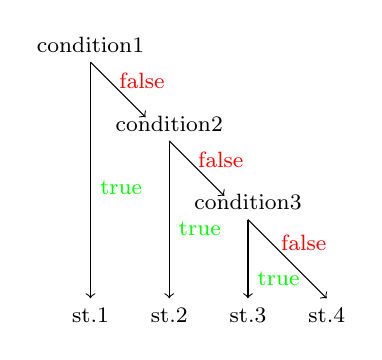
\begin{tikzpicture}[font=\footnotesize]
			\node at (0,0)[above]{condition1};
			\draw[->] (0,0) -- (0,-3) node[green, above=4em, right]{true};
			\node at (0,-3)[below]{st.1};
			\draw[->] (0,0) -- (.7,-.7) node[red, above=1.3em, right=-1.3em]{false};
			
			\node at (1,-1)[above]{condition2};
			\draw[->] (1,-1) -- (1,-3) node[green, above=2.5em, right]{true};
			\node at (1,-3)[below]{st.2};
			\draw[->] (1,-1) -- (1.7,-1.7) node[red, above=1.3em, right=-1.3em]{false};
			
			\node at (2,-2)[above]{condition3};
			\draw[->] (2,-2) -- (2,-3) node[green, above=.7em, right]{true};
			\node at (2,-3)[below]{st.3};
			\draw[->] (2,-2) -- (3,-3) node[red, above=2em, right=-2em]{false};
			
			\node at (3,-3)[below]{st.4};
		\end{tikzpicture}
		\column{0.5\textwidth}
			\begin{lstlisting}[numbers=none, basicstyle=\footnotesize]
if(condition1)
   statement1;
else if(condition2)
   statement2;
else if(condition3)
   statement3;
else
   statement4;
\end{lstlisting}
	\end{columns}
\end{frame}

\begin{frame}[fragile]{Judge the Type of an Input Character (1)}

\begin{itemize}
	\item {Judge an input character is a digit, a character, space or something else}	
	\item {Steps outlined}
	\begin{enumerate}
		\item {Accept/take input character}
		\item {Check whether in digit range (`0'-`9')}
		\item {Otherwise, check whether it is in character range (`a'-`z')}
		\item {Otherwise, check whether it is in (`A'-`Z')}
		\item {Otherwise, check whether it is space (` ')}
	\end{enumerate}
	\item {Work it by yourself first...}
\end{itemize}

\end{frame}

\begin{frame}[fragile]{Judge the Type of an Input Character (2)}
\begin{lstlisting}[basicstyle=\footnotesize]
#include <stdio.h>
int main()
{
   char ch = '';
   printf("Please input a character: ");
   ch = getchar();
   printf("Character is: %c", ch);
   if(ch >= '0' && ch <= '9'){
       printf("a digit\n");
   }else if(ch >= 'a' && ch <= 'z'){
       printf("char in lower case\n");
   }else if(ch >= 'A' && ch <= 'Z'){
       printf("char in upper case\n");
   }else if(ch == ' '){
       printf("It is space\n");
   }else{
       printf("not digit, char or space\n");
   }
   return 0;
}
\end{lstlisting}

\end{frame}


\begin{frame}[fragile]{Judge whether it is a leap year (1)}
\begin{itemize}
	\item {Leap year should satisfy one of follow two conditions}
	\begin{enumerate}
		\item {It is dividable by 4, but not by 100}
		\item {It is dividable by 400}
	\end{enumerate}
\end{itemize}

[Steps]
\begin{enumerate}
	\setcounter{enumi}{0}
	\item {Accept input number}	
	\item {Check whether it is dividable by 400}
	\item {If yes, it is leap year}
	\item {Otherwise, check whether it is dividable by 4 and NOT dividable by 100}
	\begin{enumerate}
	\setcounter{enumi}{4}
	\item {If yes, it is leap year}
	\item {Otherwise, it is not leap year}
	\end{enumerate}
\end{enumerate}
Give your solution first....
\end{frame}

\begin{frame}[fragile]{Judge whether it is a leap year (2)}
\vspace{-0.1in}
\begin{lstlisting}[basicstyle=\footnotesize]
#include <stdio.h>
int main()
{
   int year = 0, leap = 0;
   printf("Please enter the year: ");
   scanf("%d", &year);
   if(year%400 == 0){
       leap = 1;
   }else if(year%4 == 0 && year%100 != 0){
          leap = 1;
   }else{
       leap = 0;
   }
   if(leap == 1){
       printf("%d is leap year\n", year);
   }else{
       printf("%d is not leap year\n", year);
   }
}
\end{lstlisting}

\end{frame}

\begin{frame}[fragile]{More about if-else clause (1)}
\begin{itemize}
	\item {See the result of following code}
\end{itemize}
\begin{lstlisting}
int main()
{  
   int a = 3, b = 5, c = 3;
   if(a != 3)
   if(b > 9)
     printf("b = %d", b);
   else 
     printf("c = %d", c);
   return 0;
}
\end{lstlisting}
\end{frame}

\begin{frame}[fragile]{More about if-else clause (2)}
\begin{itemize}
	\item {See the result of following code}
\end{itemize}
\begin{columns}
\begin{column}{0.48\linewidth}
\begin{lstlisting}[xleftmargin=0.05\linewidth]
int main()
{  
   int a = 3, b = 5;
   int c = 3;
   if(a != 3)
   if(b > 9)
     printf("b = %d", b);
   else 
     printf("c = %d", c);
   return 0;
}
\end{lstlisting}
\end{column}
\begin{column}{0.5\linewidth}
\begin{lstlisting}[xleftmargin=0.05\linewidth]
int main()
{  
   int a = 3, b = 5, c = 3;
   if(a != 3)
   {
      if(b > 9)
       printf("b = %d", b);
      else 
       printf("c = %d", c);
   }
   return 0;
}
\end{lstlisting}
\end{column}
\end{columns}
\end{frame}

\begin{frame}[fragile]{A few words on style}
	\begin{itemize}
		\item {Do not put statements and conditions on the same line}
	\end{itemize}
	\begin{lstlisting}[numbers=none]
if(cond){ statement; }	/* bad style */

if(cond){		/* looks better, still bad style */
    statement;
}

if(cond)
	statement;   /* It is OK but not recommnended, put {} all the time */
\end{lstlisting}
\end{frame}

\begin{frame}[fragile]{More words on style}
	\begin{itemize}
		\item {Inside an \textcolor{blue}{if}-\textcolor{blue}{else} structure}
		\item {Put all blocks of this structure in braces}
	\end{itemize}
\begin{lstlisting}[numbers=none]
if(cond)		/* bad style, inconsistent */
    statement;
else {
    statement;
    statement;
}
\end{lstlisting}
\vspace{-0.3in}
\begin{columns}
\begin{column}{0.45\linewidth}
\begin{lstlisting}[numbers=none]
if(cond){  
  /* way better style */
  statement;
}else{
  statement;
  statement;
}
\end{lstlisting}
\end{column}
\begin{column}{0.45\linewidth}
\begin{lstlisting}[numbers=none]
if(cond)
{
  statement;
}else
{
  statement;
  statement;
}
\end{lstlisting}
\end{column}
\end{columns}
\end{frame}


\begin{frame}[fragile]{Operator: L=a$\divideontimes$b?c:d}
\begin{itemize}
	\item {Following codes produce the same results}
\end{itemize}
\vspace{-0.15in}
\begin{columns}
\begin{column}{0.48\linewidth}
\begin{lstlisting}[xleftmargin=0.05\linewidth]
int main()
{  
   int a = 3, b = 4, c = 1;
   if(a > b)
   {
      a = c;
   }else{
      a = b;
   }
   printf("a = %d", a);
}
\end{lstlisting}
\end{column}
\begin{column}{0.48\linewidth}
\begin{lstlisting}[xleftmargin=0.05\linewidth]
int main()
{  
   int a = 3, b = 4, c = 1;
   a = a > b?c:b;
   printf("a = %d", a);
}
\end{lstlisting}
\end{column}
\end{columns}
\vspace{-0.1in}
\begin{itemize}
	\item {``a$\divideontimes$b'' is a logic expression}
	\item {If it is true, c is assigned to the left}
	\item {Otherwise, d is assigned to the left}
\end{itemize}
\end{frame}

\begin{frame}[fragile]{Application: Convert lower case char to upper case (1)}
\begin{itemize}
	\item {Given a char of unknown case,  convert it to uppercase}
	\item {`a'-`z' to `A'-`Z'}
	\item {Solution:}
	\begin{enumerate}
		\item {Check whether \textbf{ch} is in the range of `a'-`z'}
		\item {If it is in this range, ch = ch - 32}
		\item {Otherwise, do not do anything}
	\end{enumerate}
\end{itemize}
\end{frame}

\begin{frame}[fragile]{Application: Convert lower case char to upper case (2)}
\begin{columns}
\begin{column}{0.5\linewidth}
\begin{lstlisting}[basicstyle=\footnotesize, xleftmargin=0.02\linewidth]
int main()
{  
   char ch = getchar();
   if(ch >= 'a' && ch <= 'z')
   {
      ch = ch - 32;
   }
   printf("ch = %c", ch);
   return 0;
}
\end{lstlisting}
\end{column}
\begin{column}{0.5\linewidth}
\begin{lstlisting}[basicstyle=\footnotesize, xleftmargin=0.02\linewidth]
int main()
{  
   char ch = getchar();
   ch = (ch>='a' && ch <='z')?(ch-32):ch;
   printf("ch = %c", ch);
   return 0;
}
\end{lstlisting}
\end{column}
\end{columns}
\begin{itemize}
	\item {It is concise}
	\item {Do not make your expression too long}
	\item {Take the left way when you are uncertain}
\end{itemize}
\end{frame}

\begin{frame}[fragile]{if clause: the last example}
\begin{columns}
\begin{column}{0.05\linewidth}
\end{column}
\begin{column}{0.48\linewidth}
\begin{lstlisting}[]
int main()
{
   int a = 3, b = 5, c = 2;
   if( a > b);
   {
      a = c;
   }
   a = a*2;
   printf("a = %d\n", a);
   return 0;
}
\end{lstlisting}
\end{column}
\end{columns}
\end{frame}

\begin{frame}[fragile]{switch-case clause (1)}
\begin{itemize}
	\item {Now you are given a new task}
	\item {Convert numbers (1-12) to Month (January - December)}
	\item {We can do it by \textcolor{blue}{if}-\textcolor{blue}{else} clause}
\end{itemize}
\vspace{-0.1in}
\begin{columns}
\begin{column}{0.05\linewidth}
\end{column}
\begin{column}{0.6\linewidth}
\begin{lstlisting}[numbers=none, basicstyle=\footnotesize]
int main()
{
   int n = 0;
   scanf("%d", &n);
   if(n == 1)
   {
     printf("January\n");
   }else if(n == 2){
     printf("Febuary\n");
   }else if(n == 3){
     printf("March\n");
   }
   ...
   ...
   ...
}
\end{lstlisting}
\end{column}
\end{columns}
\end{frame}

\begin{frame}[fragile]{switch-case clause (2)}
\begin{itemize}
	\item {Now you are given a new task}
	\item {Convert numbers (1-12) to Month (January - December)}
	\item {We can do it by \textcolor{blue}{if}-\textcolor{blue}{else} clause}
\end{itemize}
\vspace{-0.1in}
\begin{columns}
\begin{column}{0.1\linewidth}
\end{column}
\begin{column}{0.8\linewidth}
\begin{lstlisting}[numbers=none, basicstyle=\footnotesize]
int main()
{
   int n = 0;
   scanf("%d", &n);
   switch(n)
   {
     case 1: {printf("January\n"); break;}
     case 2: {printf("Febuary"); break;}
     case 3: {printf("March\n"); break;}
     case 12: {printf("December\n"); break;}
   }
   return 0;
}
\end{lstlisting}
\end{column}
\end{columns}
\end{frame}

\begin{frame}[fragile]{switch-case clause (3)}
\begin{itemize}
	\item {If you have to check one variable for many constant values}
	\item {\textcolor{blue}{switch}-\textcolor{blue}{case} is your friend:)}
\end{itemize}
	\begin{lstlisting}[numbers=none, basicstyle=\footnotesize]
switch(variable)
{
    case option1: statement1; break;
    case option2: statement2; break;
    case option3: statement3; break;
    default: statement4; break;
}
\end{lstlisting}
\begin{itemize}
	\item \textit{case option} defines a jump label
	\item More than one statement after it possible without braces
	\item All statements until the next \textcolor{red}{break;} will be executed
\end{itemize}	 
\end{frame}

\begin{frame}[fragile]{switch-case clause (4)}
\begin{itemize}
	\item {What \textcolor{red}{break} means}
	\item {Work out the output of following codes}
\end{itemize}
\vspace{-0.1in}
\begin{columns}
\begin{column}{0.1\linewidth}
\end{column}
\begin{column}{0.8\linewidth}
\begin{lstlisting}[numbers=none, basicstyle=\footnotesize]
int main()
{
   int n = 3;
   switch(n)
   {
     case 1: {printf("January\n"); }
     case 2: {printf("Febuary"); break;}
     case 3: {printf("March\n"); }
     case 4: {printf("April\n"); }
     case 5: {printf("May\n"); break;}
     case 12: {printf("December\n"); break;}
     default: break;
   }
   return 0;
}
\end{lstlisting}
\end{column}
\end{columns} 
\end{frame}

\end{document}
